\documentclass[../main.tex]{subfiles}
Unser Projekt haben wir aus den unter Punkt «2.2 Methode» geschilderten Gründen nach der Projektmethode IPERKA gegliedert.
\subsection{Informieren} \label{Informieren}
\subsubsection{Operationsbefehle} \label{Operationsbefehle}
Bei der Recherche für unsere Arbeit stiessen wir immer wieder auf Zitate, die aus einem Dokument namens «Operationsbefehl Nr. 13» stammen.
Es erschien uns, zusammen mit dem Operationsbefehl 12, der ebenfalls häufig in Erwähnung trat, als zentrale Dokumente der Verteidigungsstrategie, weshalb wir die Suche nach dem vollen Inhalt der beiden Dokumente starteten. 
Da wir auf unserer Suche im Internet nicht fündig wurden, wendeten wir uns an die Kontaktstelle des Bundes: admin.ch.
Die Antwort mit Zugangsdaten zu einem Archiv von Operationsbefehlen -- 18 an der Zahl -- erreichte uns vom eidgenössischen Departement für
Verteidigung, Bevölkerungsschutz und Sport VBS innerhalb von wenigen Tagen.

Die Befehle erhielten wir als eingescannte PDF-Dateien, weshalb wir das Lesen und das Erarbeiten einer Zusammenfassung für jeden Operationsbefehl unter den Gruppenmitgliedern aufteilten. 
Aus jedem Befehl wurden die Divisionen, deren Zusammensetzung und Position, Verschiebungen und generelle Informationen ausgelesen und in einem Word-Dokument zusammengefasst und auf einer Karte eingezeichnet.
So hatten wir alle wichtigen Informationen kurz und prägnant in einer digitalen, weiter verarbeitbaren Form.

\subsubsection{Wichtige Personen} \label{Wichtige Personen}
Um dem Besucher unserer Webseite noch etwas mehr Hintergrundinformationen zu liefern, haben wir uns entschieden, die wichtigsten Personen, die für die Strategie im Zweiten Weltkrieg verantwortlich waren, darauf darzustellen. Dazu haben wir uns im Internet über die Schweiz im Zweiten Weltkrieg mit ihren Entscheidungsträgern informiert und zu den wichtigsten Personen Notizen gemacht.

\subsubsection{Festung Vitznau} \label{Festung Vitznau}
Für uns war es wichtig, eine Festung aus dem Zweiten Weltkrieg von innen zu sehen, damit wir uns ein Bild vom Leben der Soldaten während des Krieges machen konnten.
Im Internet informierten wir uns über Festungen, die wir besuchen könnten. Wir stiessen auf die Festung Vitznau, wo uns grosszügigerweise eine komplette Führung unentgeltlich offeriert wurde. Erich Steiner führte uns dabei während rund zweier Stunden durch die Festung. Wir schossen Fotos und konnten unsere Fragen stellen.

\begin{figure}[h]
    \centering
    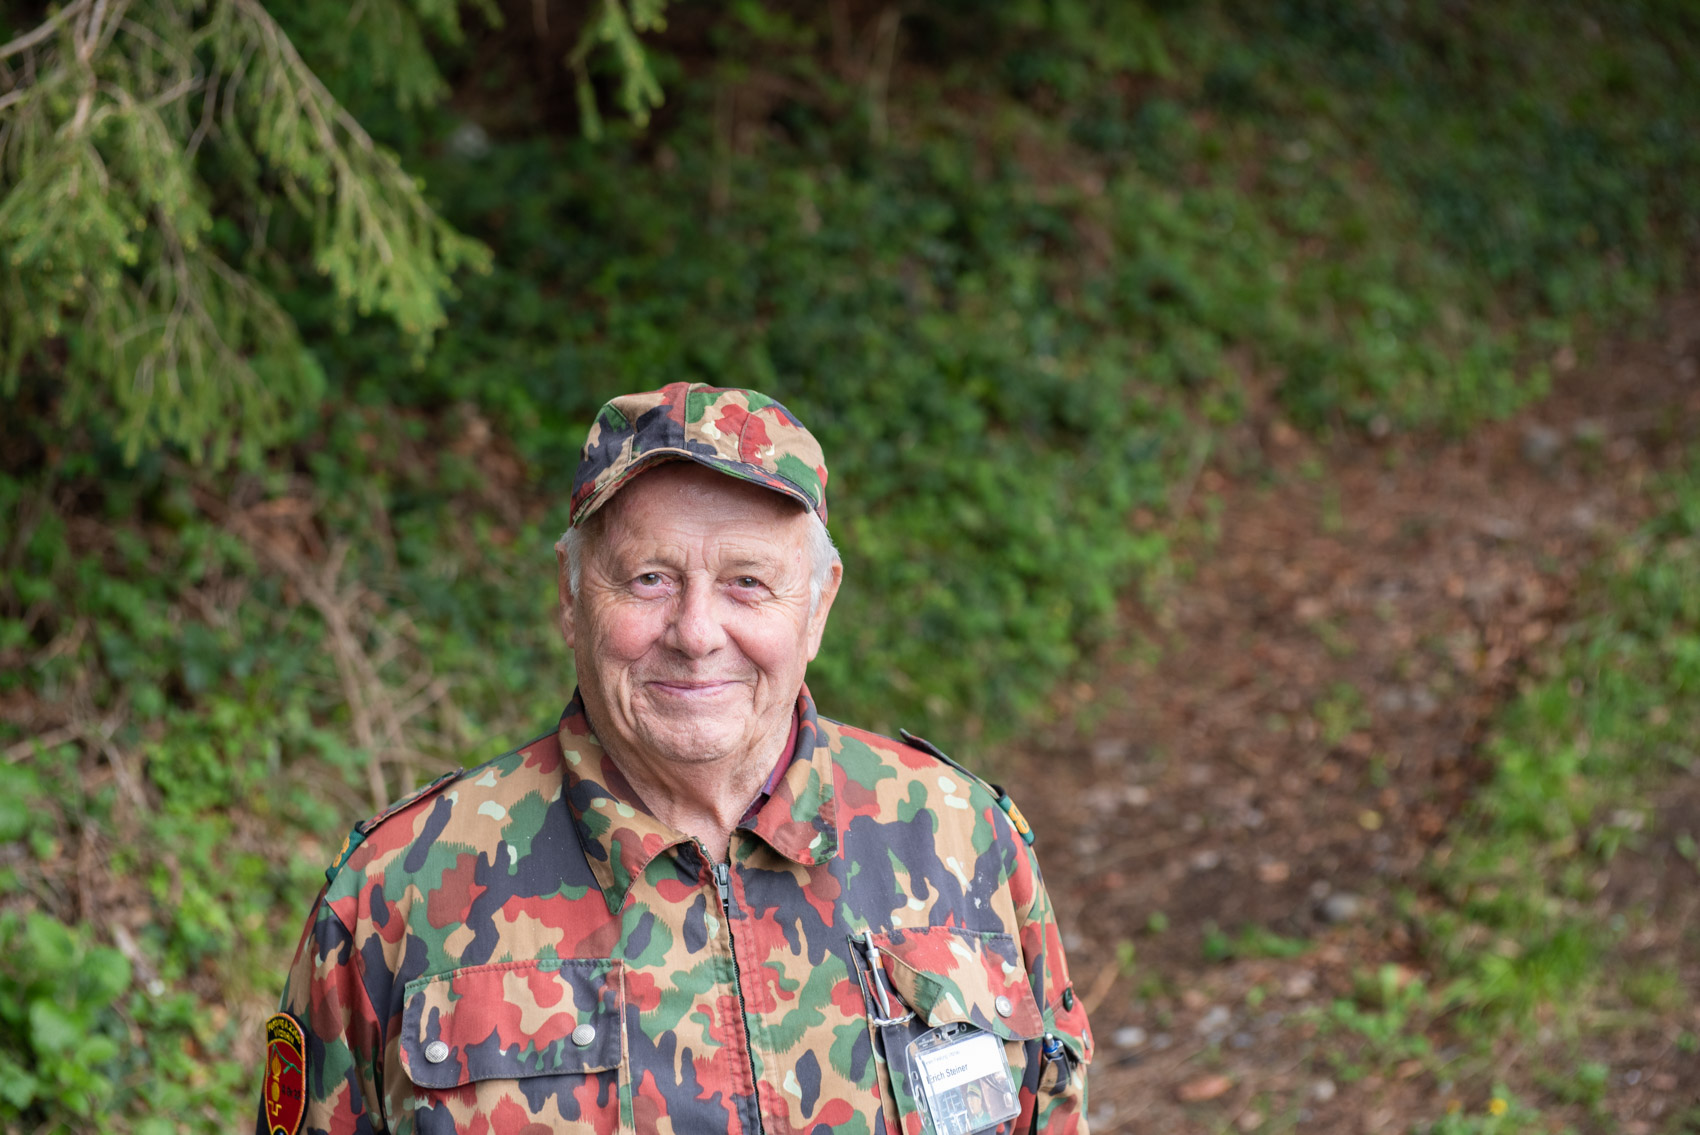
\includegraphics[width=\textwidth,height=7cm,keepaspectratio]{images/ErichSteiner.jpg}
    \caption[{Seya Schmassmann (2019). Festungsführer Erich Steiner [Stand 22.08.2019] }] {Festungsführer Erich Steiner}
\end{figure}

Nach einer kurzen Vorstellung unseres Festungsführers Erich Steiner, welcher als pensionierter Primarlehrer des öfteren Führungen anbietet und 
einer kurzen Einführung in die Eckdaten der Festung traten wir ein.
Ein kleiner, sehr unscheinbaren Eingang verband die Betongänge mit der Aussenwelt. 
Sofort standen wir in einem kleinen Eingangsbereich, welcher uns mit seinem feucht-kalten Klima auf die folgende Zeit im Bunker vorbereitete.
Ein langer Gang, schliessbar durch eine mächtige Stahltüre -- wie sie uns im Bunker noch oft begegnete -- stach uns sofort ins Auge. 
Daneben befand sich eine Schiessvorrichtung, welche für Eindringlinge, die sich Zugang über den Haupteingang verschaffen wollten, ausgelegt war. 
Wir begaben uns in den Gang und begegneten nach den ersten hundert Metern einer Gedenkstätte. 
Die heilige Barbara, als Schutzpatronin für sämtliche Arbeiten im Untertagebau, war hier platziert. 

Die Krümmung im Hauptgang der Festung, so belehrte uns Erich Steiner, sei eine Sicherheitsvorrichtung gewesen. 
Ein Gegner wurde so abgehalten vom Eingang direkt in die gesamte Festung schiessen zu können. 
Wir liefen weitere hundert Meter den Gang empor und wurden von Erich Steiner angehalten, als ein Gang Richtung rechts führte, in welchen wir schliesslich auch abbogen. 
Herr Steiner führte uns den seitlichen Gang neben den Regalen, gefüllt mit Gewehren und Helmen, vorbei in die Festungs-Werkstätte. 
Wir erfuhren, dass sämtliche Reparaturarbeiten durch die in diesem Raum vorhandenen Werkzeuge vorgenommen werden konnten. 
Angeschlossen an die Werkstätte waren die Stromgeneratoren, welche die Festung rundum mit Elektrizität versorgen könnten. 
Stolz startete Herr Steiner einen der drei Generatoren und meinte, dass durch ihre Wartung alle noch lauffähig seien. 

Weiter, vorbei am Heizungsraum und Vitrinen mit ausgestellten Gasmasken, standen wir vor einer weiteren Stahltüre.
Ein kleines Glasfenster verriet uns bereits, was als Nächstes anstand: der Unterkunftstrakt. 
Die Wärme des einzig beheizten Raumes der Festung spürte man sofort. Ebenfalls fielen die zahlreichen Bilder an den Wänden auf. 
Sie sollten den Soldaten die langen Wartezeiten im Bunker so erträglich wie möglich gestalten und einen geringen Ersatz zu den fehlenden Fenstern darstellen. 
Wir stiegen die Treppe hoch zu den Bettschlägen und begannen mit dem tiefsten Dienstgrad. Gegen die 30 Mann fanden in den Zimmern Platz. 
Mit steigendem Dienstgrad erhob sich auch der Komfort und sank die Zimmergrösse. 
So endeten wir bei einem Doppelzimmer für den Kommandanten. Zurück im ersten Stockwerk wurde uns noch das Festungsspital gezeigt. 
Im Speisesaal hing prominent der Schweizer General Guisan an der Wand; er sei von den Soldaten sehr geschätzt worden, sagte man uns. 
Die Küche war zum Teil noch mit originalen Utensilien bestückt, wobei für das Bewirten der Gäste auch Geschirrspülmaschinen vorhanden waren. 
Wie es sich vorzustellen lässt, bestanden die Speisen zu einem Grossteil aus Kartoffeln und Essen aus den Konserven, da den Zutaten eine lange Haltbarkeit abverlangt wurde. 
Wir saugten die interessanten Informationen regelrecht auf und verliessen den Aufenthaltstrakt wieder.

Zurück im Hauptgang liefen wir ans Ende der Festung, stoppten jedoch noch zweimal, um die beiden grossen Munitionslager zu besichtigen. 
40 Tonnen Schiesspulver befand sich ehemals darin. Der Spannungsbogen der gesamten Führung erhob sich beim Besichtigen der Schiessstände nochmals. 
Während des Schiessens hatte das Tragen der Schutzmasken als Pflicht gegolten. 
Die Schiessanlage wurden glücklicherweise nie gebraucht. 

Ein weiterer Höhepunkt bot der Wachposten, mit seinem einzigen Guckloch nach draussen. 
Es misst 10 Zentimeter im Durchmesser und war für die Soldaten die einzige Möglichkeit das Tageslicht zu sehen. Mit dem Verlassen der Festung endete unsere Führung.

Was uns am meisten erstaunte, war die benötigte Belegschaft, die für das Bedienen von zwei Kanonen notwendig gewesen war. 
Zudem stellten wir uns das Ausharren in den düsteren Teilen der Festung zusammen mit der gesamten weiteren Belegschaft als sehr anstrengend vor und 
verspürten Hochachtung von den Soldaten, welche dies durchgestanden hatten. Und über einen weiteren Punkt waren wir uns alle einig: 
Erich Steiner hätten wir nicht zuletzt wegen seiner sehr humorvollen Art noch sehr lange zuhören können. 

\subsubsection{Festungen} \label{Festungen}
Das Herzstück der Schweizer Verteidigungsstrategie im 2. Weltkrieg sind die zahlreichen Festungseinrichtungen, verteilt in der ganzen Schweiz.
Natürlich interessierte uns in erster Linie die Positionierung der Festungen. Eine Suche nach einer Karte mit den lange geheimgehaltenen Bunkersystemen verlief erfolglos. Folglich erweiterte die Idee, selber eine Karte der Festungen zusammenzustellen, unser Produkt.
Mithilfe einer Liste der Bunker von Wikipedia, der Webseite festung-oberland.ch und Google Maps konnten wir die Positionen der Festungen ermitteln.

\subsection{Planen} \label{Planen}
Die Vielzahl an Informationen, die wir zusammentragen konnten, mussten geschickt und auch für Benutzer, die mit dem Thema bisher wenig Berührung hatten, verständlich auf unsere Webseite gegliedert werden. Da die Strategie der Schweiz im Zweiten Weltkrieg der Fokus unserer Webseite und somit unseres Projektes sein sollte, stellten wir eine interaktive Schweizerkarte, auf welcher ein User die verschiedenen Truppen der verschiedenen Operationsbefehle ein- und ausblenden kann, in den Fokus. Zudem beinhaltete unsere ursprüngliche Idee einer interaktiven Karte auch das Anzeigen der Gefahren des Auslandes – so könnte man die Truppenverteilung der Schweiz besser nachvollziehen. Eine Übersicht über die grössten und wichtigsten Bunker ist einer zweiten Ansicht der Schweizer Karte zu entnehmen.
Die Fotos der Festung Vitznau wollten wir mit Text versehen und in einer Art Diashow auf der Webseite abbilden. Damit die Übersicht über die Vielzahl an Fotos nicht verloren geht, hilft ein Grundriss der Festung die Fotos der richtigen Stelle des Bunkers zuzuordnen.
Wir planten, die für die Entstehung der Strategien und des Reduitsplanes verantwortlichen Personen zu porträtieren.

Zu Beginn des Projektes mussten wir einen Zeitplan erstellen, was wir mit Excel gemacht haben. Die Verfeinerung mit der Aufteilung der Aufgaben wurde mit dem Onlinetool Clickup.com vorgenommen.

\subsection{Entscheiden} \label{Entscheiden}
Nach Abschluss der Planungsphase mussten wir Entscheide über den Inhalt unserer praktischen Arbeit treffen. Wir entschieden uns dazu, die Webseite in drei Teile aufzuteilen: die wichtigsten Personen, eine ausführliche Ansicht der Festung Vitznau und die Schweizerkarte mit den Operationsbefehlen und Bunkern.

Im Verlauf unserer Planung bemerkten wir jedoch, dass wir beim letzten der drei Punkte – der interaktiven Karte – einige Einbussen einstecken werden müssen, da die uns zu diesem Zeitpunkt vorgeschwebte Karte jeglichen Rahmen des Machbaren gesprengt hätte. Dies war einerseits auf einige technische Gründe zurückzuführen, welche im Kapitel «4.4.2 Technische Umsetzung» erwähnt werden, andererseits fehlten uns Informationen und die Zeit, diese mit Recherchearbeiten zu suchen, um die Gefahren des Auslandes aufführen zu können.

\subsection{Realisieren} \label{Realisieren}

\subsubsection{Dokumentation} \label{Dokumentation}
Die Dokumentation der IDPA wurde mit der Technologie LaTeX und im Editor VsCode geschrieben.

\subsubsection{Technische Umsetzung} \label{Technische Umsetzung}
Wir werden in diesem Punkt bewusst die technische Umsetzung nur oberflächlich betrachten, da eine komplette Aufarbeitung der eingesetzten Frameworks den Rahmen an dieser Stelle sprengen würde.

Bei der Wahl der Technologien für die technische Umsetzung der Webseite mussten wir sicherstellen, dass die Technologie auf verschiedenen Betriebssystemen läuft, da drei unserer Gruppenmitglieder einen Windows-Laptop und ein Mitglied ein MacBook nutzen.
Wir haben uns entschieden, das JavaScript Framework Angular zu verwenden, da es für einen solchen Auftrag geeignet ist und einige der Gruppe bereits mit dieser oder ähnlichen Technologien Erfahrungen gesammelt haben.
Alle Daten, welche auf der Webseite dargestellt werden, befinden sich in verschiedenen JSON-Dateien, welche einfach erklärt lediglich für die Datenhaltung eingesetzt werden.

Die Hauptschwierigkeit lag darin, eine Karte der Schweiz mit den Bunkern und den Truppenverteilungen zu erstellen, welche nützliche Funktionen wie das Zoomen und Anzeigen der Ortsnamen unterstützt. Dafür hätten wir gerne eine externe Library eingesetzt, welche uns die gesamte Karte mit ihrem kompletten Funktionsumfang bereitgestellt hätte. Dieser Bereich war für uns alle jedoch komplettes Neuland, weshalb wir uns einigten, die Schweizerkarte lediglich als Bild auf die Webseite zu laden und die Informationen darüber abzubilden.

\subsection{Kontrollieren} \label{Kontrollieren}
Zu kontrollieren gab es sowohl die schriftliche Arbeit als auch das Produkt, also die erstellte Webseite. Die schriftliche Arbeit kontrollierten wir einerseits durch die Verwendung des Rechtschreibe-Programmes von Microsoft Word, andererseits gaben wir die Arbeit mehreren Personen zum Korrekturlesen.
Die Webseite kontrollierten wir, indem wir sie von verschiedenen Benutzern testen liessen und ihr Feedback verarbeiteten.

\subsection{Auswerten} \label{Auswerten}
Zum Schluss des Projektes haben wir unsere Fragestellungen beantwortet und ein Fazit aus unserer Arbeit gezogen. Die Auswertung befindet sich unter dem Punkt «6 Diskussion».

